\section{Data Diversity Leads to Generalization}
\label{sec:data_diversity}
Our experiments thus far have linked training stability to rule commitment. In this section, we will show that models can, in fact, stabilize without a systematic rule---if they memorize their training instead. Less diverse training data produces models that stabilize through memorization, whereas more diverse training data produces models that commit to systematic rules. Furthermore, mirroring our previous findings in data complexity, intermediate levels of data diversity lead to highly unstable runs even when all examples induce the same rule. 
\subsection{Measuring Data Diversity}
\label{sec:data_diveristy}

We define the diversity of a dataset according to the syntactic similarity between different examples. 
We measure a sentence pair's similarity by the tree-edit distance (TED) of their latent tree representations \citep{Chomsky2015-bg}. When two sentences share the same syntax tree, transforming one into the other requires only leaf-node (i.e., vocabulary) changes. For example, \textit{My unicorn entertains her tyrannosaurus}, and, \textit{Your zebra eats some apples}, have different vocabulary but identical syntax trees. We define a dataset's diversity as the number of unique syntactic trees it contains. Similar methods are used to measure diversity in both natural language \citep{Huang2023-ab, Gao2024-fi, Ramirez2022-mx} and code \citep{Song2024-cg}. 

\subsection{Diversity and stability}
\label{sec:inverse}

We will next show that when the model is exposed to fewer unique syntax trees during training, it memorizes their patterns without reliably applying rules to unseen structures. We demonstrate the effect by designing datasets to induce either hierarchical or linear generalization and then adjusting adjusting the syntactic diversity of representative examples. Whichever rule is induced, diversity imposes three distinct regimes: stable memorization behavior at low diversity, stable generalization behavior at high diversity, and unstable behavior at intermediate levels. This transition, from stable to unstable to back to stable, forms a U-shaped curve of stability with respect to dataset diversity.

\paragraph{Hierarchy-inducing data}  
We first control data diversity on datasets that induce hierarchical generalization in QF. We construct variations of the QF training data with different levels of syntactic diversity. Each constructed training set includes 50K question samples and 50K center embedding declarations, while varying the syntactic diversity of the declaration examples. We train 50 random seeds for each modified training set and measure intra-run instability with total variation (see \ref{sec:tv_def}). To assess rule commitment, we report the proportion of runs achieving generalization accuracy either >95\% or < 5\%, indicating a commitment to either rule (here, hierarchical rule is preferred).


Figure \ref{fig:data_diversity_uscale} (\textit{left}) shows an inverse U-shaped relationship between data diversity and training instability, revealing three distinct regimes. Low-diversity data leads to the \textbf{memorization regime}, where training is stable but the model fails to commit to a rule. In Appendix \ref{appdx:memorizaition}, we confirm that models in this low-diversity regime apply the hierarchical rule to syntax structures memorized during training, but cannot extrapolate the rule to unseen  structures. High-diversity data leads to the \textbf{hierarchical generalization regime}, where training stabilizes because models commit to the hierarchical rule. In the mid-diversity \textbf{unstable regime}, the lack of data diversity hinders the likelihood of fully commiting to a rule but the data is too diverse to memorize easily. Overall, with insufficient diversity, relatively few runs learn to apply the hierarchical rule across all examples.

\paragraph{Linearity-inducing data} 
In Figure \ref{fig:intra_inter_variance} (\textit{right}), the model has a strong preference to apply the linear rule OOD when the training data contains 99\% linearity-inducing data (i.e., right branching sentences). However, Figure \ref{fig:grokking_selection} shows that when the training data contains \textit{exclusively} right-branching sentences, models do not consistently follow any systematic rule (further details in  Appendix \ref{sec:simple_mixin}). We can use data diversity to explain the failure to commit to a rule from exclusively right-branching examples: right-branching sentences lack syntactic variation, as the main auxiliary always follows the subject noun. This lack of syntax diversity prevents rule extrapolation. By introducing center embeddings in just 1\% of sentences, we introduce the diversity necessary to learn a systematic generalization rule. 

To confirm that data diversity is also key to rule commitment for when data is mostly linearity-inducing, we create variations of QF training data with 50K questions and 50K declarations, including 99\% right-branching and 1\% center-embedded sentences. We control the diversity of \textit{center-embedded} sentences as before and use the proportion of runs achieving generalization accuracy either above 95\% or below 5\% to quantify the likelihood of committing to any rule (in this data setting, linear rule is preferred). Figure \ref{fig:data_diversity_uscale} (\textit{right}) shows that training is least stable at intermediate levels of diversity, again providing three regimes: the memorization, unstable, and \textbf{linear generalization regime}.


\begin{figure}[t]
    \centering
    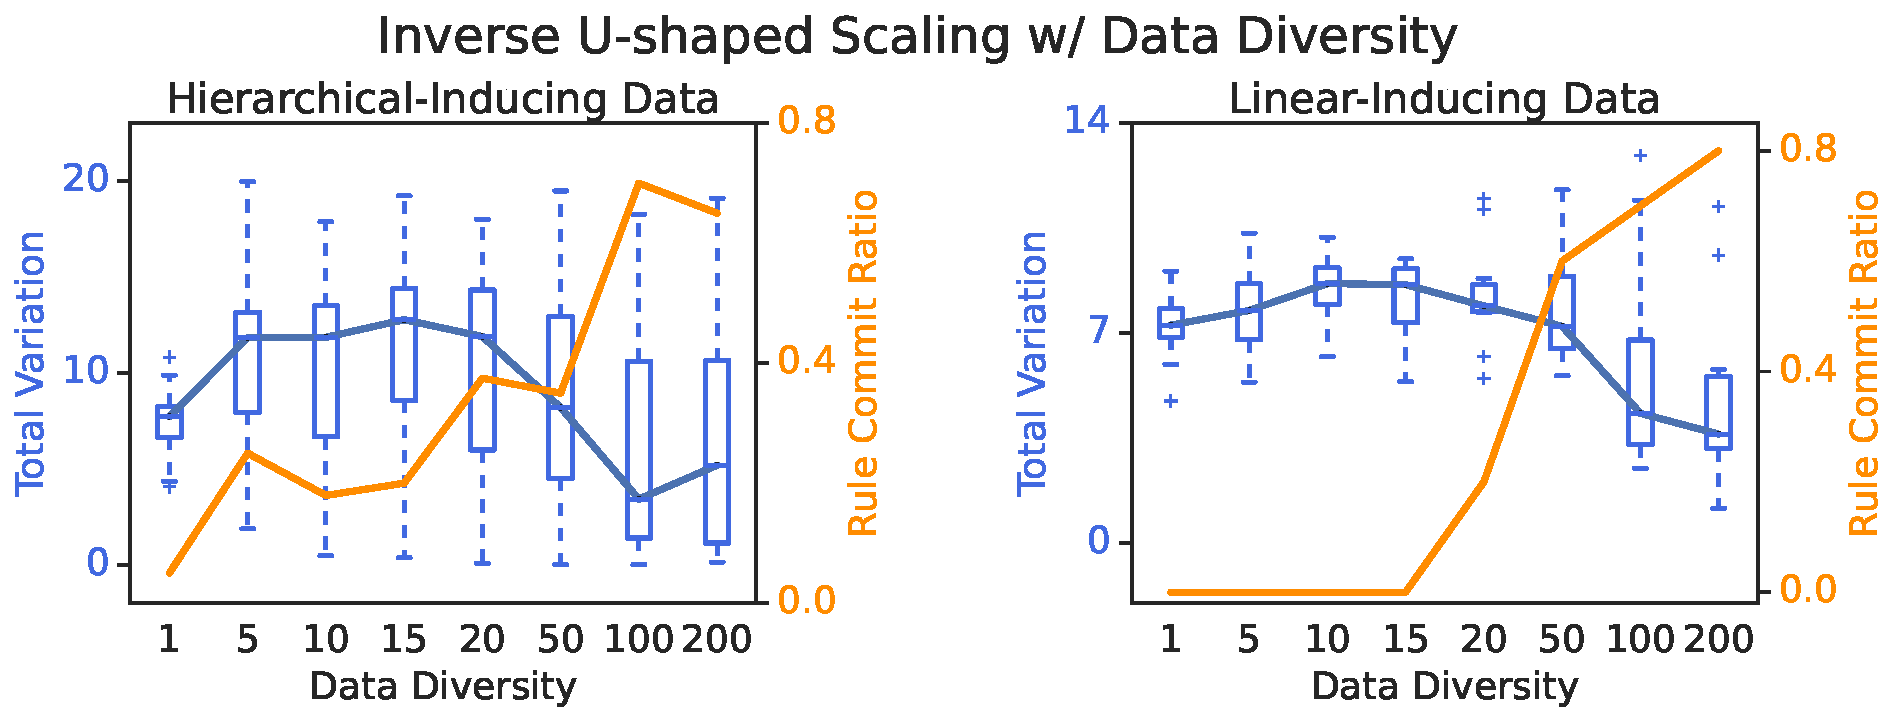
\includegraphics[width=0.8\linewidth]{figures/data_diversity_uscale.pdf}
    \caption{\textbf{Inverse U-shaped relationship between training stability and data diversity.} Whether training data favors the hierarchical (\textit{left}) or linear (\textit{right}) rule, diverse data promotes systematic rules over example memorization. At low diversity, training is stable but the model memorizes individual syntactic patterns rather than committing to a rule. With moderate data diversity, training becomes unstable. As diversity increases further, the model commits to a rule and training is the most stable.} 
    \label{fig:data_diversity_uscale}
    \vspace{-4px}
\end{figure}